\myChapter{Conclusioni}
\section{Lavori correlati}
Esistono numerosi lavori riguardanti algoritmi che tentano di imitare la produzione artistica. Uno dei più noti è \textit{Portrait drawing by Paul the robot} \cite{paul}, dove un algoritmo che controlla un braccio robotico produce schizzi su una tela con uno stile artistico programmabile per mimare il ritratto di una persona. Tramite approcci basati sul \textit{reinforcement learning} (apprendimento con rinforzo) sono state scoperte collezioni di tratti di pennello capaci di rappresentare al meglio un input fotografico dato \cite{oriental}.

Approcci basati sulle reti neurali sono stati sfruttati per sviluppare modelli generativi di immagini, anche se, come già accennato in precedenza, si è trattato più che altro di immagini in pixel e quasi mai in vettoriale. Un primo risultato ha fatto uso di \textit{Hidden Markov Models} per sintetizzare linee e curve, alcuni più recenti, introducendo l'uso di reti ricorrenti, hanno gettato le basi per l'implementazione attraverso MDN che è poi stata utilizzata per \texttt{sketch-rnn}.

Un fattore limitante per gli sviluppi di ricerca nell'ambito della generazione di disegni vettoriali è stato la mancanza di dataset disponibili pubblicamente. In precedenza lo \textit{sketch dataset} \cite{sketch}, consistente di ventimila schizzi codificati in vettoriale, era utilizzato nell'esplorazione delle tecniche di estrazione di caratteristiche. Un lavoro successivo, \textit{sketchy database} \cite{sketchy}, forniva settantamila sketch vettoriali insieme alle corrispondenti immagini in pixel per varie classi. Grazie a \textit{Quick, Draw!} adesso sono state rese disponibili milioni di immagini vettoriali suddivise in centinaia di classi diverse.

La maggiore disponibilità ha offerto lo spunto per numerose applicazioni successive che vanno da progetti artistici come \href{http://frauzufall.de/en/2017/google-quick-draw/}{\textit{Letter collages}} che delimita delle aree e usa la rete per riempirle di disegni, o \href{http://project.laboiteatortue.com/facesofhumanity/}{\textit{Faces of Humanity}} che genera volti condizionandoli rispetto a porzioni di sketch di provenienze geografiche diverse, a lavori di analisi dei dati come \href{https://qz.com/994486/the-way-you-draw-circles-says-a-lot-about-you/}{\textit{How do you draw a circle?}} che studia la provenienza culturale dell'utente osservando l'ordine dei tratti.

\begin{figure}
	\centering
	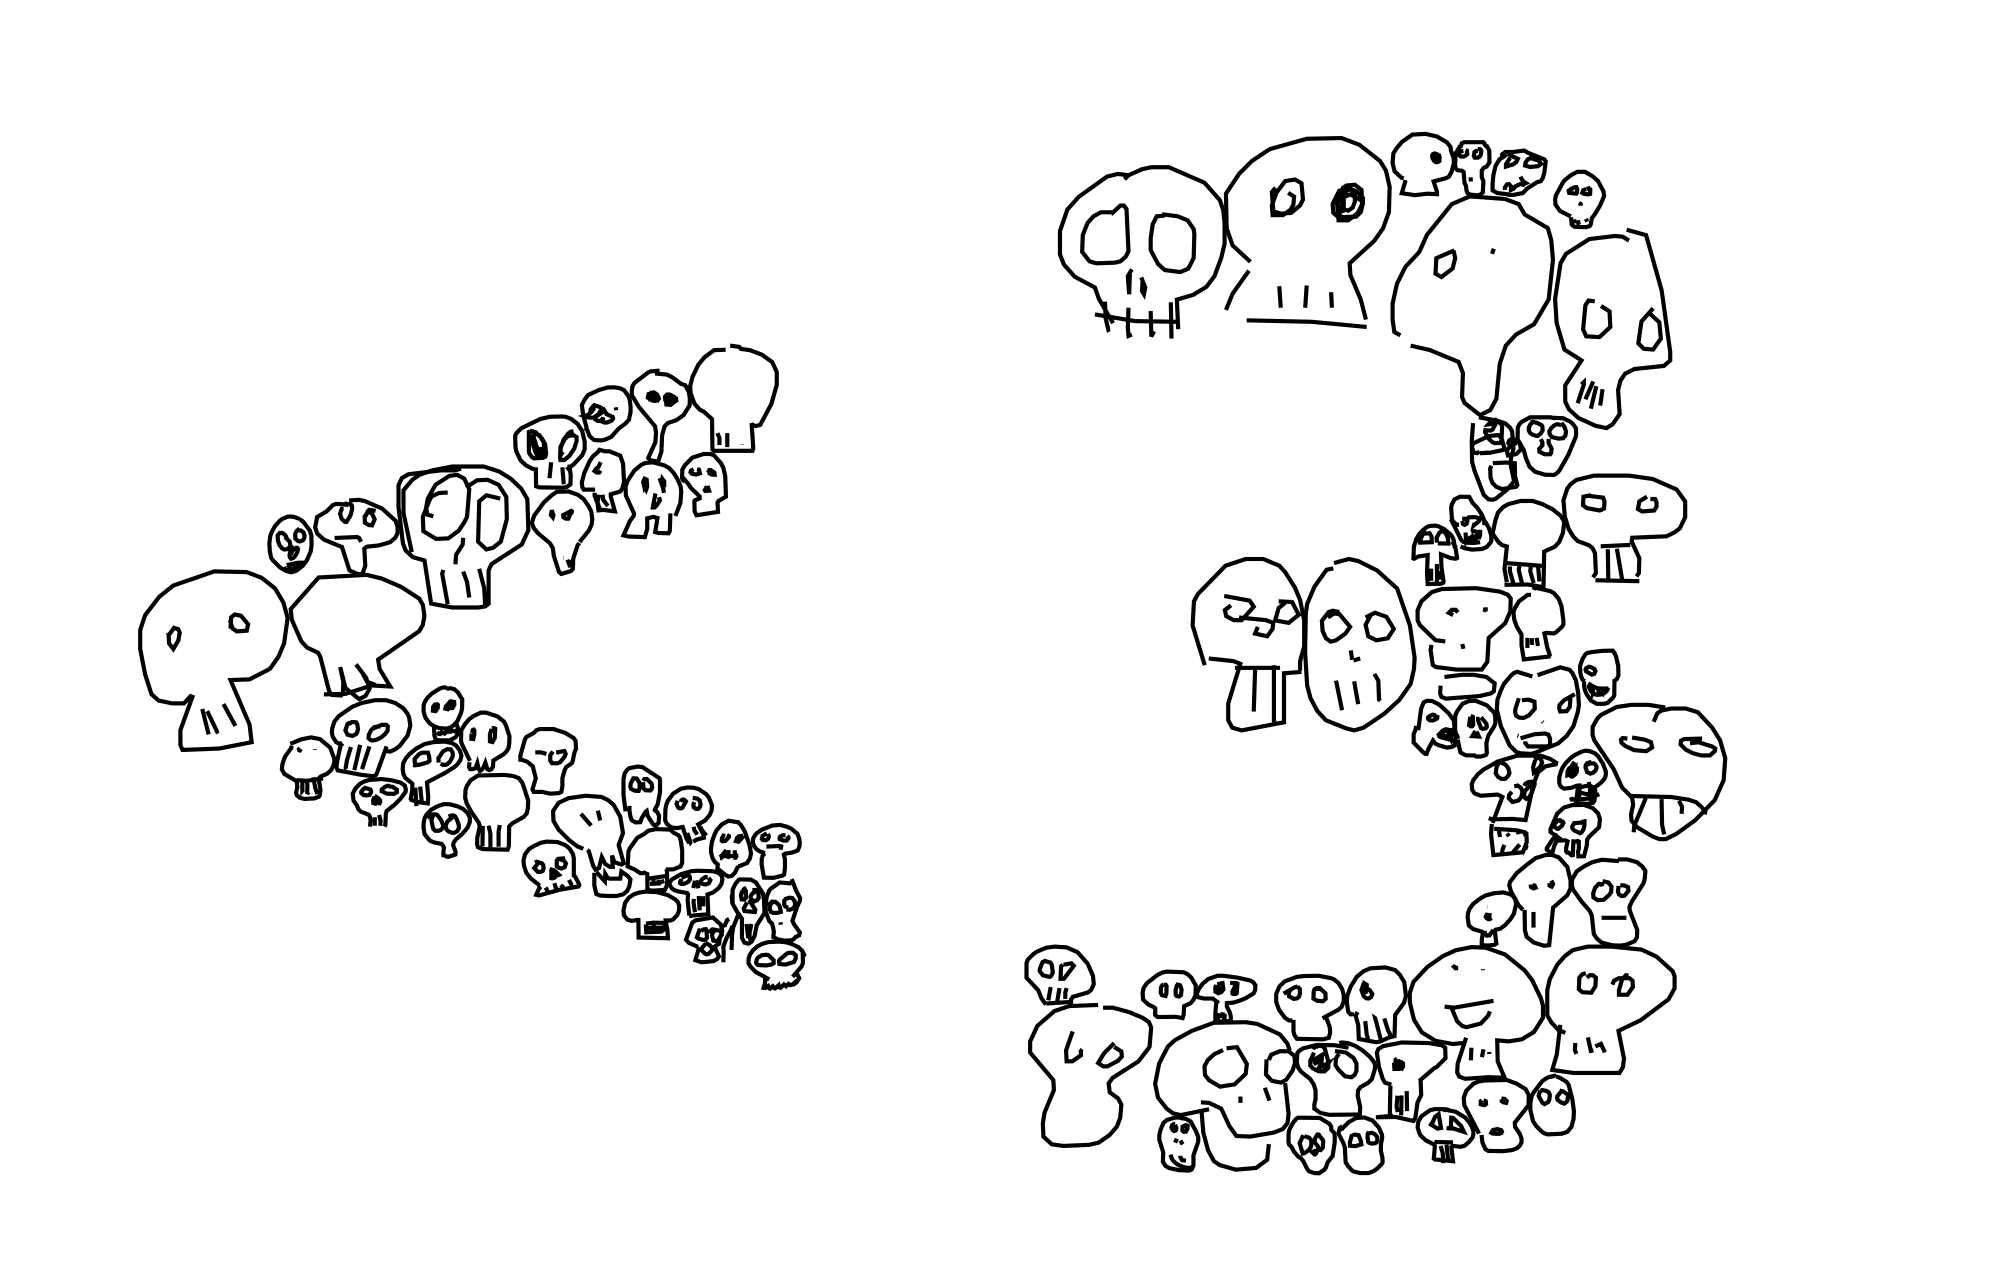
\includegraphics[width=\linewidth]{img/heart.png}
	\caption{Immagine tratta da \href{http://frauzufall.de/en/2017/google-quick-draw/}{\textit{Letter collages}}.}
	\label{img:32}
\end{figure}

\section{Sviluppi futuri} % (fold)
\label{sec:sviluppi_futuri}
\texttt{Sketch-rnn} è potenzialmente in grado di dare spunto a molte applicazioni artistiche. Come è stato mostrato, il semplice modello composto unicamente da un decoder è in grado di assistere il progetto creativo suggerendo varie opzioni possibili per completare uno schizzo abbozzato di partenza, stimolando l'immaginazione di un grafico. Nel modello condizionale esplorare lo spazio di latenza fra oggetti diversi permette di vedere interessanti combinazioni e relazioni fra forme complesse. Anche nel suo uso più semplice, un artista potrebbe sfruttare l'unicità dei disegni generati dalla rete per creare pattern articolati appartenenti ad una specifica categoria, per applicazioni tessili o stampe. Allo stesso modo il condizionamento rispetto ad uno schizzo con proprietà che la rete non conosce può offrire astrazioni interessanti, che a loro volta possono essere interpolate per produrre forme estremamente peculiari.

In futuro, un modello addestrato su schizzi di qualità superiore potrebbe assistere il processo educativo, sia offrendo rappresentazioni grafiche e semplificate dei concetti a persone con disturbi specifici dell'apprendimento, sia semplicemente guidando gli studenti più giovani nell'imparare a disegnare. Alcune applicazioni correlate riguardano la codifica di disegni di bassa qualità estetica, da migliorare utilizzando un modello con un'elevato $w_{KL}$ e una bassa temperatura \ref{sub:training}, che in futuro potrebbero implicare procedure di incrementi sul vettore di latenza che massimizzino la coerenza dei tratti, incorporando un sistema di giudizi dell'utente. Inoltre è possibile combinare variazioni ibride di modelli a generazione di sequenze con modelli generativi non supervisionati che lavorano su immagini in pixel, per dare origine a immagini fotorealistiche a partire da disegni o, all'opposto, per passare da una foto ad uno schizzo analogo.

In termini più astratti e lontani nel futuro si può osservare come nonostante le macchine sorpassino già di gran lunga le prestazioni umane, quando si tratta di percepire l'ambiente circostante con precisione, uno dei più grandi limiti che riscontrano sta nell'incapacità di interpretare concettualmente gli oggetti e le forme che stanno analizzando. I modelli generativi, che si sforzano di costruire una rappresentazione della categoria dei dati che gli vengono presentati, e in particolar modo quelli come \textit{sketch-rnn} che lavorando su immagini vettoriali si concentrano appunto sulla forma, potrebbero aprire la strada a modelli in grado, un giorno, di elaborare vere e proprie astrazioni concettuali allo stesso modo in cui è in grado di farlo un essere umano.
% section sviluppi_futuri (end)
